\nocite{*}
\chapter{Introduction} 
    

  
\chapter{Requirements} 
    The microservice will be about a calculation process for ball bearings in O-assignment. 

    \section{Flow chart for calculation process}
        Bearing A and B (Kegelrollenlager) in O-assignment. 
        
        \begin{tikzpicture}[node distance = 2cm]
            \node [terminator, fill=blue!20] (start) {\textbf{Start}};
            \node [process, fill=blue!20, below of=start] (conversion) {conversion of geometric measures};
            \node [process, fill=blue!20, below of=conversion] (radial) {calculation of radial forces};
            \node [process, fill=blue!20, below of=radial] (axial) {calculation of axial forces};
            \node [process, fill=blue!20, below of=axial] (equivalent) {calculation of dynamic equivalent bearing load};
            \node [process, fill=blue!20, below of=equivalent] (lifetime) {calculation of bearing lifetime};
            \node [data, fill=blue!20, below of=lifetime] (result) {lifetime of bearing in hours};
            \node [terminator, fill=blue!20, below of=result] (end) {\textbf{End}};

            \path [connector] (start) -- (conversion);
            % \draw [arrow] (decision) -- node[anchor=east] {yes} (conversion);
            % \draw [arrow] (decision) -- node[anchor=south] {no} (einschaltdauer);
            \path [connector] (conversion) -- (radial);
            \path [connector] (radial) -- (axial);
            \path [connector] (axial) -- (equivalent);
            \path [connector] (equivalent) -- (lifetime);
            \path [connector] (lifetime) -- (result);
            \path [connector] (result) -- (end);
        \end{tikzpicture}

        \begin{tikzpicture}
            \begin{class}[text width=8cm]{Bearing}{0,0}
                \attribute{- cdyn : double}
                \attribute{- y : double}
                \attribute{- e : double}
                \attribute{- xB1 : double}
                \attribute{- p: double}
                \attribute{- fr: double}
                \attribute{- fa: double}
                \attribute{- lh10: double}
            \end{class}
        \end{tikzpicture}

        \begin{tikzpicture}
            \begin{class}[text width=8cm]{OArrangement}{0,0}
                \attribute{- bearingA : Bearing}
                \attribute{- bearingB : Bearing}
                \attribute{- xD1 : double}
                \attribute{- xD2 : double}
                \attribute{- load: Load}
                \attribute{- a: double}
                \attribute{- b: double}
                \attribute{- c: double}  
                \attribute{- lh10: double}             
            \end{class}
        \end{tikzpicture}

        \begin{tikzpicture}
            \begin{class}[text width=8cm]{Load}{0,0}
                \attribute{- fr : double}
                \attribute{- fa : double}
                \attribute{- n : double}
                \attribute{- xr : double}
                \attribute{- ya : double}          
            \end{class}
        \end{tikzpicture}

        % \begin{tikzpicture}[node distance = 3cm]
        %     \node [terminator, fill=blue!20] (start) {\textbf{Start}};
        %     \node [data, fill=blue!20, below of=start] (data) {Provide data};
        %     \node [decision, fill=blue!20, below of=data] (decision) {Valid data?};
        %     \node [process, fill=red!20, right of=decision] (error) {Error};
        %     \node [process, fill=green!20, below of=decision] (success) {Success};
        %     \node [terminator, fill=blue!20, below of=success] (end) {\textbf{End}};
        %     \node[draw=none] at (1.70, -5.75) (no) {No};
        %     \node[draw=none] at (0.35, -7.80) (yes) {Yes};
        %     \path [connector] (start) -- (data);
        %     \path [connector] (data) -- (decision);
        %     \path [connector] (decision) -- (error);
        %     \path [connector] (decision) -- (success);
        %     \path [connector] (error) |- (end);
        %     \path [connector] (success) -- (end);
        % \end{tikzpicture}

\chapter{Prerequisites}
    The following steps and guides relate to docker container, therefore the following preparations have to be made first, otherwise the steps will not work.  

    \begin{enumerate}
        \item Install \href{https://www.docker.com/products/docker-desktop/}{Docker Desktop}
        \item Install \href{https://code.visualstudio.com/download}{Visual Studio Code} 
        \item Install the VSCode extension \href{https://marketplace.visualstudio.com/items?itemName=ms-vscode-remote.vscode-remote-extensionpack}{Remote Development} 
        \item Install the VSCode extension \href{https://marketplace.visualstudio.com/items?itemName=ms-azuretools.vscode-docker}{Docker}
    \end{enumerate}    

\chapter{How to set up Git for remote development}\label{chap:git_remote}
    This chapter is about setting up git in a Docker container. When there is no suitable container running yet, then you have to start a new one. This would be the default case. \\
    You have to open a command line interface of your choice, for example Powershell for Windows or \ac{bash} for Linux-based systems. 
    Afterwards you can go through these required steps: 
    \begin{enumerate}
        \item This command will create a container based on the image \textit{ubuntu} with the tag \textit{focal} and afterwards a \ac{bash} will be opened. You need the options -i and -t for interactive processes like a shell.
            \begin{lstlisting}[language=bash] 
docker run -it ubuntu:focal bash 
            \end{lstlisting}
        As soon as the container has been started, you end up in the corresponding \ac{bash} which you will need for the following steps.
        \item \ac{apt} is a commandline package manager for Linux-distributions and provides commands for searching and managing as well as querying information about packages. You are able to install and uninstall packages with \ac{apt}. \\
        First the package lists are re-read, afterwards git is installed. 
            \begin{lstlisting}[language=bash] 
apt update && apt install git
            \end{lstlisting}
            You can check wheather the installtion of git was successful with: 
            \begin{lstlisting}[language=bash] 
git - -version
            \end{lstlisting}
        \item \ac{gpg} is a cryptographic software suite with which you can create key pairs (public and private) and for example create signatures. We will use it to sign our commits on GitHub.
            \begin{lstlisting}[language=bash] 
apt update && apt install gpg
            \end{lstlisting}
        \item Now we will install the GitHub \ac{cli} in our container. \\
        When you configure your container from scratch, you have to execute the commands which are provided on \url{https://github.com/cli/cli/blob/trunk/docs/install_linux.md#debian-ubuntu-linux-raspberry-pi-os-apt}
        \item Create a personal access token on \href{https://github.com/settings/tokens}{Github} at least with the permissions read:org, repo and workflow. Copy the generated token and insert the following command in \ac{bash} with the substituted token: 
            \begin{lstlisting}[language=bash] 
export GH_TOKEN = <your-token>
            \end{lstlisting}   
        Now you are authenticated with your GitHub host and are able to proceed with the next step.
%         \item Afterwards you are able to authenticate with your GitHub host via the GitHub CLI. You have multiple choices to do that.  
%             \begin{lstlisting}[language=bash] 
% gh auth login
%             \end{lstlisting}   
        \item Clone the respective GitHub respository with: 
            \begin{lstlisting}[language=bash] 
gh repo clone <link-to-repo>  
            \end{lstlisting} 
            In this case the link to the repo is \textit{themaxens/ball-bearings-with-quarkus}.
        \item Configure git to create signed commits. Replace <user-name> and <email> with your own credentials. 
            \begin{lstlisting}[language=bash] 
git config gpg.program gpg && git config commit.gpgsign true
git config user.name "<user-name>"
git config user.email "<email>"
            \end{lstlisting}
        \item The next step is to create the private and public \ac{gpg} key \autocite[vgl.][]{create_gpg}.
            \begin{lstlisting}[language=bash] 
gpg --full-generate-key 
            \end{lstlisting} 
        Afterwards you are prompted to specify details for the key. Here you can accept the defaults with the exception of the key size. Enter a key size of 4096. \\
        Finally you have to specify your userid information and assign a password. 
        \item \label{itm:gpg_key} Use the following command to list the long form of the \ac{gpg} keys. 
            \begin{lstlisting}[language=bash] 
gpg --list-secret-keys --keyid-format=long 
            \end{lstlisting} 
        You get the follwing view, the expiration date may differ: 
        \begin{figure}[h]
            \centering
            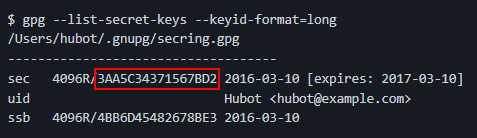
\includegraphics{images/gpg_keys.png}
            \caption{List of \ac{gpg} keys}
            \label{fig:gpg_key}
        \end{figure}
        Copy the \ac{gpg} key ID, in this case: 3AA5C34371567BD2 
        \pagebreak
        \item Enter this text with your copied ID. Your \ac{gpg} key will be printed to console.
            \begin{lstlisting}[language=bash] 
gpg --armor --export <id>
            \end{lstlisting}
        Copy the printed key, beginning with \textit{BEGIN PGP PUBLIC KEY BLOCK} and ending with \textit{END PGP PUBLIC KEY BLOCK}.  
        \item Now you are able to add the key to your GitHub Account: \url{https://github.com/settings/gpg/new}
        \item After you have added the key to GitHub, you have to tell Git your signing key. 
            \begin{lstlisting}[language=bash] 
git config --unset gpg.format
            \end{lstlisting}   
        The \textit{--global} is not necessary in this case. The settings are only made for the current repository you are in. \\
        Use the same \ac{gpg} key id as  in \ref{itm:gpg_key} and enter this command. 
            \begin{lstlisting}[language=bash] 
git config user.signingkey <id>
            \end{lstlisting}   
        You can configure Git to sign all commits by default with:
            \begin{lstlisting}[language=bash] 
git config commit.gpgsign true
            \end{lstlisting} 
        From now on, your local commits will be signed.   
        \item Last but not least you have to configure the .bashrc file. It is a startup configuration file for the \ac{bash} which is loaded every time a terminal is opened. The export command will set the environment variable \textit{GPG\_TTY} to the correct terminal so that the passphrase for your \ac{gpg}-key can be queried correctly. The export command will be attached  to the .bashrc file in your home directory.  
            \begin{lstlisting}[language=bash] 
[ -f ~/.bashrc ] && echo 'export GPG_TTY=$(tty)' >> ~/.bashrc
            \end{lstlisting}
    \end{enumerate}
    Once you have successfully completed all the steps, Git is configured in the Docker container. 

    \section{Attach Visual Studio Code to Docker Container}
        Open VSCode and navigate to the Docker-symbol in the vertical-left bar as shown in figure \ref{fig:attach_vscode}. \\
        When Docker Desktop is running, you will see all your containers. Maybe you have to start the container first. \\
        Peform a right click on the respective container and select \glqq Attach Visual Studio Code\grqq. 
        \begin{figure}[h]
            \centering
            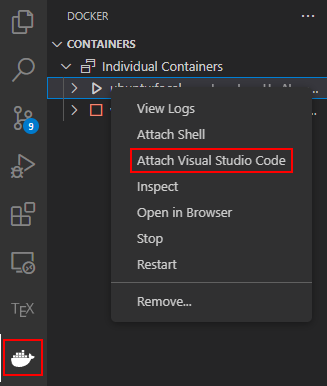
\includegraphics[scale=0.7]{images/attach_VSCode.png}
            \caption{Attach Docker Container to VSCode}
            \label{fig:attach_vscode}
        \end{figure}
        
        Afterwards the container will be attached to VSCode, which can be seen by the green information in the bottom left corner. In figure \ref{fig:container_attached} you can see an example. The text may vary, depending on your image and container name.     
        
        \begin{figure}[h]
            \centering
            
\includegraphics{images/container_attached.png}
            \caption{Docker Container is attched}
            \label{fig:container_attached}
        \end{figure}
    


\chapter{How to set up Quarkus for remote development}
    This chapter is about setting up Quarkus in a Docker container \autocite[vgl.][]{quarkus}. If you have already completed the steps from chapter \ref{chap:git_remote}, you can continue with this container. Otherwise, you have to create a new container.

    \begin{enumerate}
        \item Install curl because it will be needed in future steps.
        \begin{lstlisting}[language=bash] 
apt-get update; apt-get install -y curl
        \end{lstlisting}
        \item Now you are able to install Quarkus via curl.
        \begin{lstlisting}[language=bash, breaklines=true] 
curl -Ls https://sh.jbang.dev | bash -s - trust add https://repo1.maven.org/maven2/io/quarkus/quarkus-cli/
        \end{lstlisting}

        \begin{lstlisting}[language=bash, breaklines=true] 
curl -Ls https://sh.jbang.dev | bash -s - app install --fresh --force quarkus@quarkusio
        \end{lstlisting}

        \item When you initially set up Quarkus, you have to create a new Quarkus application. In this case a getting started application would be created in the folder \textit{code-with-quarkus}. You are able to specify parameters to define the build system, for example Maven or Gradle. For more information about the available parameters, execute quarkus create app --help.
        \begin{lstlisting}[language=bash, breaklines=true] 
quarkus create && cd code-with-quarkus
        \end{lstlisting}
        \item Set \textit{quarkus.http.host} to 0.0.0.0 in application.properties under src/main/resources.
        \item Now you are able to run your application with:
        \begin{lstlisting}[language=bash]
quarkus dev
        \end{lstlisting}
        When you start the application in dev mode, live coding is active which means that you don't have to restart the application to apply changes.
    \end{enumerate}


\chapter{Implementation}


\chapter{Conclusion} % Fazit

